% Metódy inžinierskej práce

\documentclass[10pt,twoside,slovak,a4paper]{article}

\usepackage[slovak]{babel}
%\usepackage[T1]{fontenc}
\usepackage[IL2]{fontenc} % lepšia sadzba písmena Ľ než v T1
\usepackage[utf8]{inputenc}
\usepackage{graphicx}
\usepackage{url} % príkaz \url na formátovanie URL
\usepackage{hyperref} % odkazy v texte budú aktívne (pri niektorých triedach dokumentov spôsobuje posun textu)
\usepackage{cite}
%\usepackage{times}
\usepackage{graphicx}
\pagestyle{headings}

\title{Agilné postupy pri vývoji medicínskeho softvéru} 
\author{Irina Makarova\\[2pt]}
\date{}

\begin{document}
\renewcommand{\abstractname}{\vspace{-\baselineskip}} %removes abstract heading
\maketitle

\begin{abstract}
V súčasnosti sa rýchlo vyvíja trh zdravotníckych prenositeľných zariadení. Vodopádový model, ktorý sa klasicky používal pri vývoji bezpečnostne kritického softvéru, už pre svoju zdĺhavosť a nepružnosť nepredstavuje optimálny postup. Do popredia sa dostávajú rôzne agilné a kombinované prístupy, čo prináša so sebou otázku, ako implementovať do procesu vývoja agilné metódy a pri tom dodržať požadované normy. Tento článok prináša stručný prehľad aktuálne platných noriem; vysvetľuje podstatu vodopádového a agilných modelov (Scrum, XP, DSDM), porovnáva ich a poukazuje na črty jednotlivých stratégií, ktoré sú prínosné pre túto oblasť. V článku sa uvádzajú niektoré existujúce riešenia, ako sa tieto modely dajú efektívne kombinovať pri vývoji medicínskeho softvéru.
\end{abstract}

\section{Úvod} \label{uvod}
skuska citovania\cite{mccaffery2019}
\section{Prehľad noriem}
\section{Modely vývoja softvéru}
\subsection{Vodopádový model}
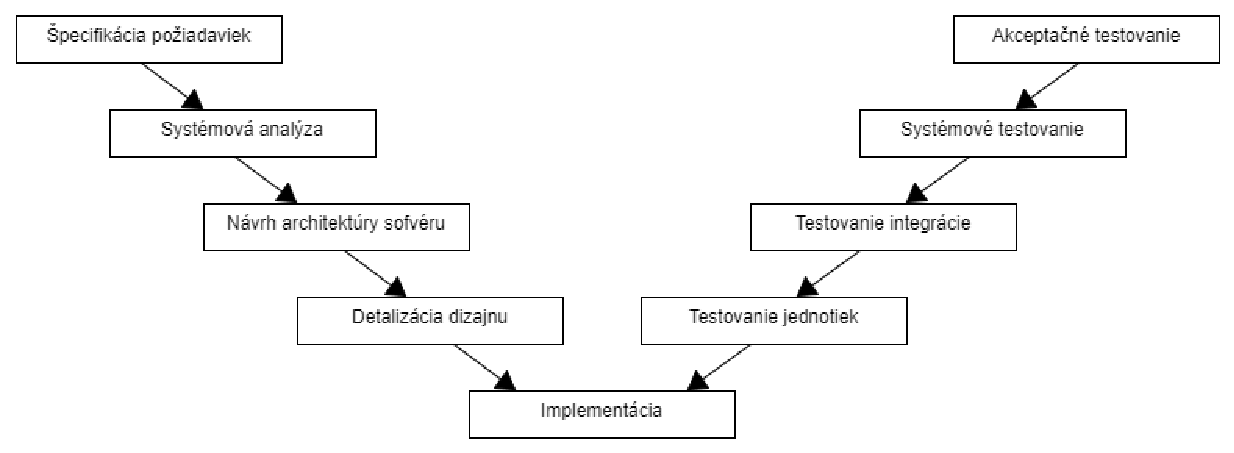
\includegraphics[width=15cm, height=8cm]{V-model.pdf}
\subsection{Agilné metódy}
\subsubsection{Scrum}
\subsubsection{Extreme programming}
\subsubsection{Dynamic System Development Method}
\section{Porovnanie vodopádového a agilných modelov}
\section{Kombinované prístupy pri vývoji medicínskeho softvéru}
\section{Záver}



% generuje zoznam literatúry z obsahu súboru literatura.bib
\bibliography{literatura}
\bibliographystyle{plain} % alpha/ abbrv/ plain
\end{document}
